\documentclass[aspectratio=169]{beamer}
\usepackage{amsmath}
\usepackage{graphicx}
% \usepackage{oz}
\usepackage{zed-csp}
\usepackage[utf8]{inputenc}
\usepackage{newunicodechar} % For defining new Unicode characters
% The listings package supports many different programming languages
\usepackage{listings}

\usetheme{Madrid}
\definecolor{UBCblue}{rgb}{0.04706, 0.13725, 0.26667}
\usecolortheme[named=UBCblue]{structure}

% Listings Configuration
\definecolor{codegreen}{rgb}{0,0.6,0}
\definecolor{codegray}{rgb}{0.5,0.5,0.5}
\definecolor{codepurple}{rgb}{0.58,0,0.82}
\definecolor{backcolour}{rgb}{0.95,0.95,0.92}

\lstdefinestyle{mystyle}{
backgroundcolor=\color{backcolour},   
commentstyle=\color{codegreen},
keywordstyle=\color{magenta},
numberstyle=\tiny\color{codegray},
stringstyle=\color{codegreen},
basicstyle=\ttfamily\footnotesize,
breakatwhitespace=false,         
breaklines=true,                 
captionpos=b,                    
keepspaces=true,                 
numbers=left,                    
numbersep=5pt,                  
showspaces=false,                
showstringspaces=false,
showtabs=false,                  
tabsize=2
}

\lstset{style=mystyle}

\newlength{\trianglewidth}
\settowidth{\trianglewidth}{\(\vartriangleleft\)}

\newcommand{\lefttrianglebar}{%
    \mathrel{\makebox[\trianglewidth]{%
        \makebox[\trianglewidth]{\(\vartriangleleft\)}%
        \hspace*{-\trianglewidth}%
        \makebox[\trianglewidth]{\(-\)}%
    }}%
}
\newcommand{\righttrianglebar}{%
    \mathrel{\makebox[\trianglewidth]{%
        \makebox[\trianglewidth]{\(-\)}%
        \hspace*{-\trianglewidth}%
        \makebox[\trianglewidth]{\(\vartriangleright\)}%
    }}%
}

\title{CS4211: Formal Methods for Software Engineering}
\subtitle{Lecture Notes}
\author{Kevin Toh}
\date{}

\begin{document}

% Slide 1
\begin{frame}
\titlepage
\end{frame}

% Slide 2
\begin{frame}{Introduction to Formal Methods}
    \begin{itemize}
        \item Requirements are difficult to define because its written in \textbf{Natural Language} which can be imprecise and ambiguous at times.
        \item As we cannot anticipate the ways a system may be used, written test cases only covers a small subset of use cases.
        \item We want to verify if a system always satisify a certain property, in possible all cases.
        \item In Formal Methods, we use \textbf{Mathematics} to define the \textbf{structure} and \textbf{behaviour} of our software because it is \textbf{precise} and \textbf{unambiguous}
        \item Eventually, we can use a model checker to automatically verify the software by checking if a certain property holds in all cases.
    \end{itemize}
\end{frame}

% Slide 3
\begin{frame}{The Z Specification Language}
    \begin{itemize}
        \item Based on set theory and mathematical logic
        \begin{itemize}
            \item We will be doing a recap on predicates, set theory, functions and relations next.
        \end{itemize}
        \item Uses schemas to declare object properties
        \begin{itemize}
            \item Schemas are similar to defining the structure of a class and its properties in an Object-Oriented Programming Language.
        \end{itemize}
        \item Uses operations to describe state transitions
        \begin{itemize}
            \item Each object has a state representing the values it's properties hold at a certain moment in time.
            \item Operations are similar to methods of a class. 
            \item Operations modify the state of an object.
            \item We use predicates to describe state transitions in an operation.
        \end{itemize}
        \item We can then proof that a certain property holds manually
    \end{itemize}
\end{frame}

% Slide 4
\begin{frame}[fragile]
\frametitle{Latex Setup}
\begin{itemize}
\item The Latex package that we will be using is \texttt{zed-csp}
\item \textbf{Setup Code: }
\begin{lstlisting}[language=tex]
% For latex document
\documentstyle[12pt,zed]{article}

% For beamer slides
\usepackage{zed-csp}  

\begin{document}
\end{document}
\end{lstlisting}
\item \href{https://sg.mirrors.cicku.me/ctan/macros/latex/contrib/zed-csp/zed2e.pdf}{Reference: https://sg.mirrors.cicku.me/ctan/macros/latex/contrib/zed-csp/zed2e.pdf}
\end{itemize}
\end{frame}

% Slide 5
\begin{frame}{Recap on Predicates and Logic}
    \begin{block}{Predicate}
        A statement that is either true or false.
        \begin{enumerate}
            \item There are 365 days in 2024. (\textbf{false})
            \item Let $P(x, y)$ be $x + y = 9$
            \begin{itemize}
                \item $P(4, 5)$ is \textbf{true}.
                \item $P(3, 7)$ is \textbf{false}.
            \end{itemize}
        \end{enumerate}
    \end{block}
    \begin{block}{Logic Operators}
        \begin{enumerate}
            \item Not ($\neg$) Eg: 
            \item And ($\wedge$)
            \item Or ($\vee$)
            \item Implies ($\implies$)
            \item Equivalence ($\iff$)
        \end{enumerate}
    \end{block}
\end{frame}

% Slide 6
\begin{frame}{Recap on Quantifiers}
    \begin{enumerate}
        \item Universal Quantifier ($\forall$)
        \begin{itemize}
            \item Example: All natural numbers are greater than -1.
            \item Mathematically, we would write $\forall n \in \nat, n > -1$
            \item In Z Specification, we would write $\forall n : \nat \spot n > -1$
            \item $\forall n : \nat \spot n > 0$
            \item In general, $\exists x : X \spot P(x)$ abbreviates $P(a) \wedge P(b) \wedge P(c) \wedge \ldots$
        \end{itemize}
        \item Existential Quantifier ($\exists$)
        \begin{itemize}
            \item Example: There exists a natural number more than 0.
            \item In Z Specification, we would write $\exists n : \nat \spot n > 0$
            \item In general, $\exists x : X \spot P(x)$ abbreviates $P(a) \vee P(b) \vee P(c) \vee \ldots$
        \end{itemize}
    \end{enumerate}
    \begin{block}{Differences between Mathematical Notations and Z Specification}
        \begin{itemize}
            \item In Mathemical Notation, : or $\mid$ means "such that" when used in Set Expressions.
            \item In Z Specification, : means "belongs to".
            \begin{itemize}
                \item The difference between : and $\in$ will be explained later.
            \end{itemize}
            \item In Z Specification, $\spot$ means "such as" when writing predicates.
        \end{itemize}
    \end{block}
\end{frame}

% Slide 7
\begin{frame}{Recap on Set Theory}
    \begin{itemize}
        \item A set is a collection of elements (or members)
        \begin{itemize}
            \item Elements are not ordered: $\{a, b, c\} = \{b, a, c\}$
            \item Elements are not repeated" $\{a, a, b\}= \{a, b\}$
            \item Given Sets
            \begin{itemize}
                \item $\nat = \{0, 1, 2, 3, \ldots \}$ (The set of all natural numbers)
                \item $\nat_{1} = \{1, 2, 3, \ldots \}$
                \item $\num = \{0, 1, -1, 2, -2, \ldots \}$ (The set of all integers)
                \item $\mathbb{R}$ (The set of all real numbers)
                \item $\emptyset$ (Empty Set: The set with no elements)
            \end{itemize}
        \end{itemize}
        \item Membership: $x \in \mathbb{X}$ is a predicate which is
        \begin{itemize}
            \item true if x is in the set $\mathbb{X}$. Eg: $a \in \{a, b, c\}$
            \item false if x is not in the set $\mathbb{X}$. Eg: $d \in \{a, b, c\}$
        \end{itemize}
    \end{itemize}

    \begin{block}{Difference between ':' and '$\in$'}
        Example: $\forall x : \num \spot x > 5 \implies x \in \nat$
        \begin{itemize}
            \item $x : \num$ declares a new variable $x$ of type $\num$
            \item $x \in \nat$ is a predicate which is either true or false depending on the value of the declared $x$.
        \end{itemize}
    \end{block}
\end{frame}

% Slide 8
\begin{frame}{Recap on Set Theory}
    \begin{itemize}
        \item Set Expressions
        \begin{itemize}
            \item We can express a set by listing its elements if the set is finite and small.
            \begin{itemize}
                \item $\{a, b, c, d\}$ is a finite set.
            \end{itemize}
            \item If a set is large or infinite, we can definite a set by giving a predicate which specifies precisely those elements in a set.
            \begin{itemize}
                \item $\nat$ is an infinite set.
                \item The set of natural numbers less than 99 is $\{n : \nat \mid n < 99\}$
                \item In general the set $\{x : \mathbb{X} \mid P(x)\}$ is the set of elements of $\mathbb{X}$ for which predicate $P$ is true.
            \end{itemize}
        \end{itemize}
        \item Set Examples
        \begin{itemize}
            \item The set of even integers is $\{z : \num \mid \exists k : \num \spot z = 2k\}$
            \item The set of natural numbers which when divided by 7 leave a remaineder of 4 is $\{n : \nat \mid \exists m : \nat \spot n = 7m + 4 \}$
            \item $\nat$ is the set $\{z : \num \mid z \geq 0\}$
            \item $\nat_1$ is the set $\{n : \nat \mid n \geq 1\}$
            \item If $a, b$ are any natural numbers, then $a \upto b$ is defined as the set of all natural numbers between a and b inclusive.
            \begin{itemize}
                \item $a \upto b$ is the set $\{n : \nat \mid a \leq n \leq b\}$
            \end{itemize}
        \end{itemize}
    \end{itemize}
\end{frame}

% Slide 9
\begin{frame}{Recap on Set Theory}
    \begin{itemize}
        \item Subset ($\subseteq$): If $S$ and $T$ are sets, $S \subset T$ is a predicate equivalent to $\forall s : S \spot s \in T$.
        \begin{itemize}
            \item The following predicates are true:
            \begin{itemize}
                \item $\{0, 1, 2\} \subseteq \nat$
                \item $2 \upto 3 \subseteq 1 \upto 5$
                \item $\{a, b\} \subseteq \{a, b, c\}$
                \item $\emptyset \subseteq X$ for any set $X$
                \item $\{x\} \subseteq X \iff x \in X$
            \end{itemize}
        \end{itemize}
        \item Proper Subset ($\subset$): If $S$ and $T$ are sets, $S \subset T$ is a predicate equivalent to $S \subseteq T \wedge S \neq T$.
        \item Power Set ($\power$): If $X$ is a set, $\power$ $X$ (the power set of $X$) is the set of all subsets of $X$.
        \begin{itemize}
            \item $A \in$ $\power$ $B$ $= A \subseteq B$ 
            \item The following predicates are true:
            \begin{itemize}
                \item $\power\{a, b\} = \{\emptyset, \{a\}, \{b\}, \{a, b\}\}$
                \item $\power$ $\emptyset$ $= \{\emptyset\} \neq \emptyset$
                \item $1 .. 5 \in \power$ $\nat$
                \item $2 .. 5 \in \power(1 .. 5)$
            \end{itemize}
            \item If $X$ has $k$ elements, then $\power$ $X$ has $2^{k}$ elements.
        \end{itemize}
    \end{itemize}
\end{frame}

% Slide 10
\begin{frame}{Recap on Set Theory}
    \begin{itemize}
        \item Set Operations
        \begin{itemize}
            \item Set Union: Suppose $S, T : \power X$ or $S \subseteq X, T \subseteq X$, then $S \cup T = \{x : X \mid x \in S \vee x \in T\}$
            \begin{itemize}
                \item $\{a, b, c\} \cup \{b, g, h\} = \{a, b, c,g, h\}$
                \item $A \cup \emptyset = A$ (for any set $A$)
            \end{itemize}
            \item Set Intersection: Suppose $S, T : \power X$, then $S \cap T = \{x : X \mid x \in S \wedge x \in T\}$ 
            \begin{itemize}
                \item $\{a, b\} \cap \{b, c\} = \{b\}$
                \item $\{a, b, c\} \cap \{d, g\} = \emptyset$ (disjoint sets)
                \item $A \cap \emptyset = \emptyset$ (for any set $A$)
            \end{itemize}
            \item Set Difference: Suppose $S, T : \power X$, then $S - T = \{x : X \mid x \in S \wedge x \not \in T\}$ 
            \begin{itemize}
                \item $\{a, b, c\} - \{b, g, h\} = \{a, c\}$
                \item $\nat_{1} = \nat = \{0\}$
            \end{itemize}
            \item Cartesian Product: If $A$ and $B$ are sets, then $A \cross B$ is the set of all ordered pairs $(a, b)$ with $a \in A$ and $b \in B$.
            \begin{itemize}
                \item $\{a, b\} \cross \{a, c\} = \{(a, a), (a, c), (b, a), (b, c)\}$
            \end{itemize}
            \item Cardinality: $\#X$ is a natural number denoting the cardinality of (number of elements in) a finite set $X$.
            \begin{itemize}
                \item $\#\{a, b, c\} = 3$
            \end{itemize}
        \end{itemize}
    \end{itemize}
\end{frame}

% Slide 11
\begin{frame}{Recap on Relations}
    \begin{itemize}
        \item A relation $R$ from sets $A$ to $B$, is declared as $R : A \rel B$ is a subset of $A \cross B$
        \item Example: $R = \{(c, x), (c, z), (d, x), (d, y), (d, z)\}$
        \begin{itemize}
            \item The following predicates are equivalent
            \begin{enumerate}
                \item $(c, z) \in R$
                \item $c \fun z \in R$
                \item $cRz$
            \end{enumerate}
        \end{itemize}
        \item \textbf{Domain:} $\dom R$ is the set $\{a : A \mid \exists b : B \spot a R b\}$
        \item \textbf{Range:} $\ran R$ is the set $\{b : B \mid \exists a : A \spot a R b\}$
    \end{itemize}
\end{frame}

% Slide 12
\begin{frame}
    \frametitle{Types in Z Specification}
    \begin{itemize}
        \item Z specification language is \textbf{strongly typed}.
        \item Every expression is given a type.
        \item Any set can be used as a type.
        \item The following are equivalent declarations of variables $x$ and $y$ of types $A$ and $B$ respectively. 
        \begin{itemize}
            \item $(x, y) : A \cross B$
            \item $x: A, y: B$
            \item $x, y : A$ (only when $B = A$)
        \end{itemize}
    \end{itemize}
\end{frame}

% Slide 13
\begin{frame}[fragile]
\frametitle{Modelling using Z Specification}
\begin{itemize}
\item When we write a program, we can write code procedurally, functionally or in an object oriented manner.
\item Z Specification can help us model our code using two distinct sections.
\begin{enumerate}
    \item Declaration: To define variables.
    \item Predicate: Often used to define behaviours or invariants.
\end{enumerate}
\item \textbf{Example \#1:} We can define the relation \textbf{divides} between two natural numbers.

\texttt{| divides: $\nat_1 \rel \nat$ \\
| ----------------------------------------- \\
| $\forall x : \nat_1; y: \nat \spot x$ \underline{divides} $y \iff \exists k : \nat \spot x \cdot k = y$}

Usage: 3 \underline{divides} 6, $\lnot$ (3 \underline{divides} 7)

\item \textbf{Example \#2:} We can define the relation $\leq$ between two natural numbers.

\texttt{| $\_<=\_$: $\nat \rel \nat$ \\
| ----------------------------------------- \\
| $\forall x, y: \nat \spot x <= y \iff \exists k : \nat \spot x + k = y$}

The relation $<=$ is the infinite subset of ordered pairs in $\nat\cross\nat$.
\\$\{(0, 0), (0, 1), (1, 1), (0, 2) (1, 2), (2, 2), \ldots \}$
\end{itemize}
\end{frame}

% Slide 14
\begin{frame}{Domain and Range Restriction}
\begin{itemize}
    \item Let $A, B, R, S, T$ be sets.
    \item $A$ is the domain set, $B$ is the range set and $R$ is the relation set.
    \item Note that $S$ is a subset of the domain set and $T$ is the subset of the range set.
    \item Suppose $R: A \rel B, S \subseteq A$ and $T \subseteq B$.
    \begin{itemize}
        \item \textbf{Domain Restriction:} $S \dres R$ is the set $\{(a, b): R \mid a \in S\}$
        \item \textbf{Range Restriction:} $R \rres T$ is the set $\{(a, b): R \mid b \in T\}$
    \end{itemize}
    \item Notice that both $S \dres R \in A \rel B$ and $R \rres T \in A \rel B$, meaning that both domain restriction and range restrictions are relations from sets $A$ to $B$.
    \item If has\_sibling: People $\rel$ People then
    \begin{itemize}
        \item female $\dres$ has\_sibling is the relationship is\_sister\_of.
        \item has\_sibling $\rres$ female is the relationship has\_sister.
    \end{itemize}
\end{itemize}
\end{frame}

% Slide 15
\begin{frame}{Domain and Range Subtraction}
\begin{itemize}
    \item Let $A, B, R, S, T$ be sets.
    \item $A$ is the domain set, $B$ is the range set and $R$ is the relation set.
    \item Note that $S$ is a subset of the domain set and $T$ is the subset of the range set.
    \item Suppose $R: A \rel B, S \subseteq A$ and $T \subseteq B$.
    \begin{itemize}
        \item \textbf{Domain Subtraction:} $S \lefttrianglebar R$ is the set $\{(a, b): R \mid a \not \in S\}$
        \item \textbf{Range Subtraction:} $R \righttrianglebar T$ is the set $\{(a, b): R \mid b \not \in T\}$
    \end{itemize}
    \item The following predicates are true.
    \begin{itemize}
        \item $S \lefttrianglebar R = (A - S) \dres R$
        \item $R \righttrianglebar T = R \rres (B - T)$
        \item $S \lefttrianglebar R \in A \rel B$
        \item $R \righttrianglebar T \in A \rel B$
    \end{itemize}
    \item If has\_sibling: People $\rel$ People then
    \begin{itemize}
        \item female $\lefttrianglebar$ has\_sibling is the relationship is\_brother\_of.
        \item has\_sibling $\righttrianglebar$ female is the relationship has\_brother.
    \end{itemize}
\end{itemize}
\end{frame}

% Slide 16
\begin{frame}{Relational Image}
\begin{itemize}
    \item Suppose the relation $R : A \rel B$ and $S \rel A$
    \item $R \limg S \rimg = \{b : B \mid \exists a : S \spot a R b\}$
    \item $R \limg S \rimg \rel B$
    \item Example
    \begin{itemize}
        \item $divides \limg \{8, 9\} \rimg = \{x : \nat \mid \exists k : \nat \spot x = 8 \cdot k \vee 9 \cdot k \} = \{0, 8, 9, 16, 18, \ldots\}$
        \item $<= \limg {3, 7, 21} \rimg = \{x : \nat \mid x >= 3\}$ 
    \end{itemize}
    \item In summary, the relational image returns the set of all elements $b \in B$ such that there exists an $a \in S$ with $(a, b) \in R$.
    \item The difference between relational image and range restriction is that range restriction returns the subset of $R$ which are ordered pairs of $(a, b)$ where $a \in A$ and $b \in B$ and the first element $a$ of the ordered pair is in $S$. The relational image simply just returns the set of all second elements $b$.
\end{itemize}
\end{frame}

% Slide 17
\begin{frame}{Inverse and Relational Composition}
    \begin{itemize}
        \item \textbf{Inverse:} $R^{-1}$ is the set $\{(b, a) : B \cross A \mid a R b \}$ or $R^{-1} \in B \rel A$
        \begin{itemize}
            \item $has\_sibling^{-1} = has\_sibling$ 
            \item $divisor^{-1} = has\_divisor$ 
        \end{itemize}
        \item Example: $succ^{-1}$ = pred
        \\ \texttt{| succ: $\nat \rel \nat$
        \\|--------------------------------------
        \\| $\forall x, y : \nat \spot x$ \underline{succ} $y \rel x + 1 = y$ 
        }
        \item \textbf{Relational Composition ($\comp$)}
        \begin{itemize}
            \item Suppose $R: A \rel B$ and $S: B \rel C$ are two relations.
            \item $R \comp S = \{(a, c) : A \cross C \mid \exists b : B \mid a R b \wedge b S c\}$
            \item $R \comp S \in A \rel C$
        \end{itemize}
        \item Examples
        \begin{itemize}
            \item $is\_parent\_of \comp is\_parent\_of = is\_grandparent\_of$
            \item $R^{0} = id[A]$
            \item $R^{1} = R$
            \item $R^{2} = R \comp R$
            \item $R^{3} = R \comp R \comp R$
        \end{itemize}
    \end{itemize}
\end{frame}

% Slide 18
\begin{frame}{Recap on Functions}
    \begin{itemize}
        \item A (partial) function from a set $A$ to a set $B$, denoted by $f: A \pfun B$ is a subset $f$ of $A \cross B$ with the property that for each $a \in A$, there is \textbf{at most one} $b \in B$ with $(a, b) \in f$.
        \item \textbf{$\dom f$} is the set $\{a : A \mid \exists b : B \spot (a, b) \in f\}$
        \item \textbf{$\ran f$} is the set $\{b : B \mid \exists a : A \spot (a, b) \in f\}$
        \item Suppose $f: A \pfun B$ and $a \in \dom f$, then $f(a)$ denotes the unique image $b \in B$ that $a$ is mapped to by $f$.
        \item $(a, b) \in f$ is equivalent to $f(a) = b$
        \item \textbf{Total Function:} If the function $f: A \pfun B$ is a total function, then $f: A \rightarrow B$ if and only if $\dom f = A$
    \end{itemize}
\end{frame}

% Slide 19
\begin{frame}{Function Overriding}
    \begin{itemize}
        \item Suppose $f, g: A \pfun B$, then $f \oplus g$ is the function $(\dom g \lefttrianglebar f) \cup g$.
        \item The following predicates are true:
        \begin{enumerate}
            \item $\dom f \oplus g = \dom f \cup \dom g$
            \item $a : \dom g$ $\spot (f \oplus g)(a) = g(a)$
            \item $\forall a : \dom f - \dom g \spot (f \oplus g)(a) = f(a)$
            \item f $\oplus$ g $\in a \pfun b$
        \end{enumerate}
        \item Examples
        \begin{enumerate}
            \item $\{a \rightarrow x, b \rightarrow y, c \rightarrow x\} \oplus \{a \rightarrow y\} = \{a \rightarrow y, b \rightarrow y, c \rightarrow x\}$
            \item double $\oplus$ root = $\{(0, 0), (1, 1), (2, 4), (3, 6), (4, 2), \ldots\}$ (Note: $(4, 8)$ was replaced with $(4, 2)$ as the domain 4 is both in $f$ and $g$, so the range was replaced with $2$ that was in $g$)
        \end{enumerate}
    \end{itemize}
\end{frame}

% Slide 20
\begin{frame}
    \frametitle{Specifying Functions}
    \begin{enumerate}
        \item Using a look-up table
        \begin{itemize}
            \item If a function $f : A \pfun B$ is finite (and not too large), we can specify the function explicity by listing all pairs $(a, b)$ in the subset $A \cross B$.
            \item Example: PassportNo $\fun$ Address
            
            \begin{tabular}{c c}
                PassportNo & Address \\
                A001017 & 77 Sunset Strip \\
                $\cdots$ & $\cdots$ \\
                G707165 & 19 Mail Street
            \end{tabular}
        \end{itemize}

        \item Declaring Axioms: A function can be specified by giving a \textbf{predicate} determining which pairs $(a, b)$ are in the function.
        \begin{itemize}
            \item \textbf{Example: The root function that calculates the square root of a natural number} 
            
            \texttt{| root $\nat \pfun \nat$
            \\|--------------------------------
            \\| $\dom root = \{n : \nat \mid \exists m:\nat \spot m^{2} = n\}$
            \\| $\forall n : \dom root$ $\spot$ $(root(n))^{2} = n$}

        \end{itemize}
    \end{enumerate}
\end{frame}

% Slide 21
\begin{frame}[fragile]
    \frametitle{Specifying Functions}
    \begin{enumerate}
        \setcounter{enumi}{2}
        \item Using Recursion: For functions defined recursively in terms of itself.
        
        \texttt{| fact $\nat_1 \pfun \nat$
        \\|--------------------------------
        \\| fact(1) = 1
        \\| $\forall n : \nat_1 - \{1\} \spot fact(n) = n * fact(n - 1)$}

        \item Giving an Algorithm: A function $f : A \pfun B$ is specified by an algorithm such that given any element $a$ in the domain of $f$, the element $f(a)$ can be computed using the algorithm.
        \begin{columns}
            \begin{column}{0.4\textwidth}
\begin{lstlisting}
input n : N
var x, y: integer;
begin
    x := n; y:= 0;
    while x != 0 do
    begin
        x := x - 1; y:= y + 2
    end;
write(y)
end
\end{lstlisting}
            \end{column}
            \begin{column}{0.4\textwidth}  %%<--- here
                \texttt{| double: $\nat \fun \nat$\\
                | ------------------\\
                | $\forall n : \nat \spot double(n) = 2n$}
            \end{column}
        \end{columns}
    \end{enumerate}
\end{frame}

% Slide 22
\begin{frame}{Sequences}
    \begin{itemize}
        \item A sequence s of elements of a set $A$, denoted $s : \seq A$, is a function $s:\nat \pfun A$ where $\dom s = 1 \upto n$ for some natural number $n$.
        \item \textbf{Example}
        \begin{itemize}
            \item $<b, c, a, b>$ denotes the sequence (function) $\{1 \fun b, 2 \fun c, 3 \fun a, 4 \fun b\}$
            \item The empty sequence is denoted by $<>$
        \end{itemize}
        \item The set of all sequences of elements from $A$ is denoted as $\seq A$ and is defined to be $\seq A = \{s : \nat \pfun A \mid \exists n:\nat$ $\spot$ $\dom s = 1 \upto n\}$
        \item $\seq_1 A = \seq A - \{<>\}$ is defined as the set of non-empty sequences.
        \item Since sequences are ordered mapping, $<a, b, a> \neq <a, a, b> \neq <a, b>$
    \end{itemize}
\end{frame}

% Slide 23
\begin{frame}{Special Functions for Sequence}
    \begin{enumerate}
        \item Concatenation 
        \begin{itemize}
            \item $<a, b> \cat <b, a, c> = <a, b, b, a, c>$
        \end{itemize}
        \item Head
        \begin{itemize}
            \item \texttt{| head: $\seq_1 A \fun A$
            \\|---------------------------------
            \\|$\forall s : \seq_1 A \spot head(s) = s(1)$}
            \item $head<c, b, b> = c$
        \end{itemize}
        \item Tail
        \begin{itemize}
            \item \texttt{| tail: $\seq_1 A \fun \seq A$
            \\|---------------------------------
            \\|$\forall s : \seq_1 A \spot <head(s)>$ $\cat$ $tail(s) = s$}
            \item $tail<c, b, b> = <b, b>$
        \end{itemize}
        \item Filter
        \begin{itemize}
            \item $<a, b, c, d, e, d, c, b, a> \filter \{a, d\} = <a, d, d, a>$
            \item Filter only keeps the element in the specified set, preserves order in the original sequence and outputs a new sequence.
        \end{itemize}
        
    \end{enumerate}
\end{frame}

% Slide 24
\begin{frame}{Z Specification}
\begin{itemize}
\item As explained in an earlier slide, we can write Z Specification to formally specify requirements in \textbf{two distinct sections}
\begin{enumerate}
    \item Declaration: To define variables.
    \item Predicate: Often used to restrain the possible values of the declared variables to define behaviours or invariants.
\end{enumerate}
\item Formal Specification can be done in the form of both \textbf{axioms} and \textbf{schemas}.
\item When we were specifying functions earlier, we were formally specifying them in the form of \textbf{axioms} in the \textbf{axiom environment}.
\item Later we will introduce how to formally specify \textbf{schemas} which are used to specify relationships between variable values.
\item There are two main type of schemas in the \textbf{schema environment}
\begin{itemize}
    \item State Schema
    \item Operation Schema
\end{itemize}
\end{itemize}
\end{frame}

% Slide 25
\begin{frame}[fragile]
\frametitle{The \texttt{zed-csp} Package}
\begin{itemize}
    \item We can use the \texttt{zed-csp} package to formally specify requirements in Z Specification and render axioms and schemas them in TeX.
    \item There are \textbf{two types of environment} in the \texttt{zed-csp} package.
\end{itemize}
\begin{enumerate}
\item Axiom Environment

\begin{columns}
\begin{column}{0.4\textwidth}
\begin{small}
\begin{axdef}
limit: \nat
\where
limit \leq 65535
\end{axdef}
\end{small}
\end{column}
\begin{column}{0.6\textwidth}
\begin{lstlisting}
\begin{axdef}
    limit: \nat
    \where
    limit \leq 65535
\end{axdef}
\end{lstlisting} 
\end{column}
\end{columns}

\item Schema Environment
\begin{columns}
\begin{column}{0.4\textwidth}
\begin{small}
\begin{schema}{PhoneDB}
known: \power NAME \\ phone: NAME \pfun PHONE
\where
known = \dom phone
\end{schema}
\end{small}
\end{column}
\begin{column}{0.6\textwidth}
\begin{lstlisting}
\begin{schema}{PhoneDB}
known: \power NAME \\ phone: NAME \pfun PHONE
\where
known = \dom phone    
\end{schema}
\end{lstlisting}
\end{column}
\end{columns}
\end{enumerate}
\end{frame}

% Slide 26
\begin{frame}{State Schema}
    \begin{itemize}
        \item A \textbf{state schema} specifies a relationship between variable values
        \item It specifies a \underline{snapshot} of a system
        \item \textbf{Variables} are declared and typed in the \textbf{top part of the schema}.
        \item A \textbf{predicate (axiom)} restraining the possible values of the declared variables are given in the \textbf{bottom part of the schema.}
        \item An instance of a schema is an assignment of values to variables consistent with their type declaration and satisfying the predicate.
    \end{itemize}
\end{frame}

% Slide 27
\begin{frame}{Operation Schema}
    \begin{itemize}
        \item The state schema provides a static view of the system.
        \item To specify how the system can change, we need to specify the operation schema.
        \item An operation can be thought as taking an instance of the state schema and producing a new instance.
        \item To specify such an operation, we express as a predicate the relationship between the \textbf{instance of the state before the operation} and the \textbf{instance after the operation.}
        \begin{block}{Convention}
            \begin{itemize}
                \item The value of the state variables before the operation are denoted by \textbf{unprimed identifiers}.
                \begin{itemize}
                    \item Example: \texttt{items : seq MSG}
                \end{itemize}
                \item Values after the operation are denoted by \textbf{primed identifiers}.
                \begin{itemize}
                    \item Example: \texttt{items' : seq MSG}
                \end{itemize}
                \item Note: Let \texttt{MSG} be the set of all possible messages that can be transmitted.
            \end{itemize}
        \end{block}
    \end{itemize}
\end{frame}

% Slide 28
\begin{frame}{Case Study: A Message Buffer}
    \begin{itemize}
        \item We are going to model a message buffer to learn about \textbf{schema specification}.
        \item A message buffer stores messages within a queue data structure and operates on a first in / first out (FIFO) principle.
        \item Suppose we have a line which might be occupied by traffic, many messages join the buffer and but only the first message in the queue leaves the buffer when the line is free.
        \item The buffer may contain several messages at any time, but there is a fixed upper limit on the number of messages the buffer may contain.
        \item To model a message buffer, we minimally need the following:
        \begin{enumerate}
            \item States: Buffer (to store messages)
            \item Operations: Join (new message joins the buffer), Leave (message leaves the buffer)
        \end{enumerate}
    \end{itemize}
    \begin{center}
        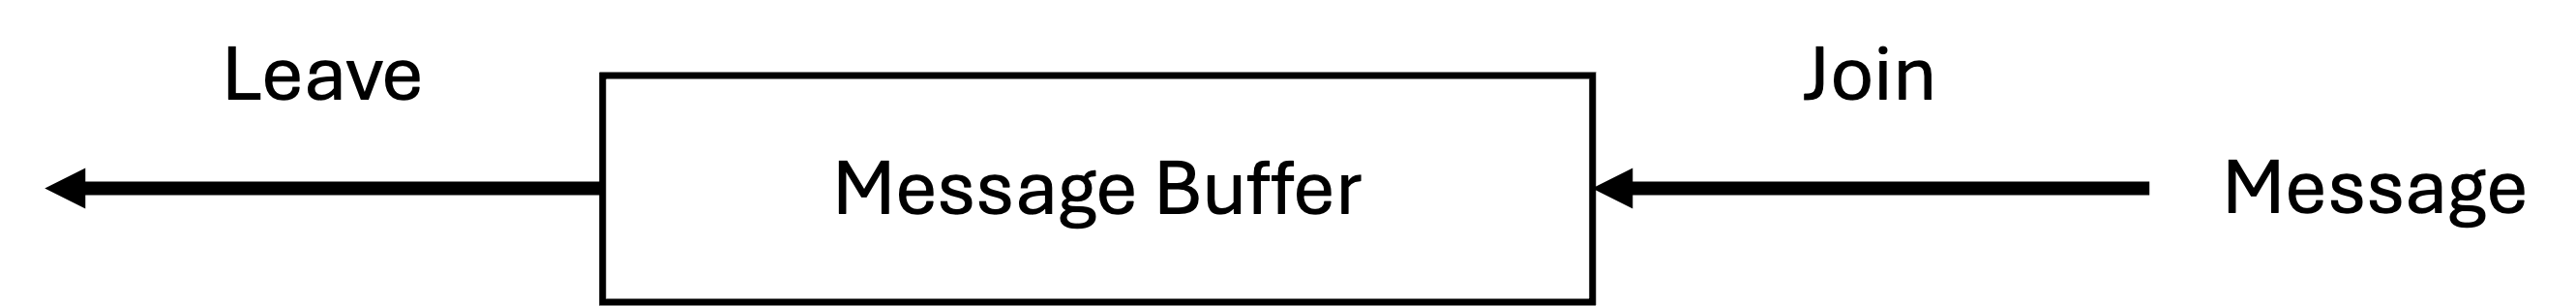
\includegraphics[scale=0.5]{../images/MessageBuffer.png}
    \end{center}
\end{frame}

% Slide 29
\begin{frame}{Formal Specification: Message Buffer}
\begin{columns}
\begin{column}{0.6\textwidth}
\textbf{State Schema: Buffer}
\begin{itemize}
    \item Let MSG be the set of all possible messages that can be transmitted.
    \item Let max : $\nat$ be the constant maximum number of messages that can be held in the buffer at any one time.
    \item Example: Let $MSG=\{m1, m2, m3\}$ and $max = 4$
    \begin{enumerate}
        \item $items = <m1, m2>$ is a valid instance.
        \item $items = <m3, m1, m1, m2, m2>$ is an invalid instance.
    \end{enumerate}
\end{itemize}
\textbf{Operation Schema: Join} 
\begin{itemize}
    \item The decoration ? denotes an input
    \item There is an implicit $\wedge$ between each line in the predicate section.
\end{itemize}
\end{column}
\begin{column}{0.4\textwidth}
\begin{small}
\begin{schema}{Buffer}
    items: \seq MSG
    \where
    \#items \leq max
\end{schema} 

\begin{schema}{Join}
    items, items': \seq MSG \\
    msg?: MSG
    \where
    \#items \leq max \\
    \#items' \leq max \\
    \#items < max \\
    items' = items \cat <msg?>
\end{schema}
\end{small}
\end{column}
\end{columns}
\end{frame}

% Slide 30
\begin{frame}{Explanation: Predicate of the Join Operation}
    \begin{columns}
        \begin{column}{0.4\textwidth}
            \begin{small}
                \begin{schema}{Join}
                    items, items': \seq MSG \\
                    msg?: MSG
                    \where
                    \#items \leq max \\
                    \#items' \leq max \\
                    \#items < max \\
                    items' = items \cat <msg?>
                \end{schema}
            \end{small}
        \end{column}
        \begin{column}{0.6\textwidth}
            \begin{itemize}
                \item The first two lines of the predicate indicate that we have a valid instance of the state schema \textbf{Buffer} both before and after the operation.
                \item The third line of the predicate is a pre-condition for the operation. It indicates that for the \textbf{Join} operation to be possible, the buffer must not be completely full.
                \item The last line of the predicate specifies the relationship between the buffer contents before and after the operation which is that the input message is already appended to the sequence of messages already in the buffer.
            \end{itemize}
        \end{column}
    \end{columns}
\end{frame}

% Slide 31
\begin{frame}{Formal Specification: Message Buffer (Continued)}
    \begin{columns}
        \begin{column}{0.63\textwidth}
            \textbf{Operation Schema: Leave}
            \begin{itemize}
                \item The decoration ! denotes an output
                \item There is an implicit $\wedge$ between each line in the predicate section.
                \item Explanation for Leave Operation Predicate
                \begin{enumerate}
                    \item The first two lines of the predicate indicate that we have a valid instance of the state schema \textbf{Buffer} both before and after the operation.
                    \item The third line of the predicate is a \textbf{pre-condition} for the operation. It indicates that for the \textbf{Leave} operation to be possible, the buffer must not be empty.
                    \item The last line of the predicate specifies the relationship between the buffer contents before and after the operation. The output message is taken from the head of the sequence of messages in the buffer, leaving just the tail of the sequence of buffers.
                \end{enumerate}
            \end{itemize}
        \end{column}
        \begin{column}{0.4\textwidth}
            \begin{schema}{Leave}
                items, items': \seq MSG \\
                msg!: MSG
                \where
                \#items \leq max \\
                \#items' \leq max \\
                \#items \neq \emptyset \\
                items = <msg!> \cat items'
            \end{schema}
        \end{column}
    \end{columns}
\end{frame}

% Slide 32
\begin{frame}{Special States: Delta ($\Delta$) and Initial State ($_{INIT}$)} 
\begin{enumerate}
\item Delta ($\Delta$): To specify a \textbf{before} and \textbf{after} instance of the state schema for any operation.
\begin{small}
\begin{schema}{\Delta Buffer}
    items, items': \seq MSG
    \where
    \#items \leq max\\
    \#items' \leq max
\end{schema} 
\end{small}
\item Initial State ($_{INIT}$): To specify a state when an instance of a state is first initialized.
\begin{columns}
    \begin{column}{0.25\textwidth}
        \begin{small}
            \begin{schema}{Buffer_{INIT}}
                Buffer
                \where
                items = <>
            \end{schema} 
            \end{small}
    \end{column}
    \begin{column}{0.75\textwidth}
        \begin{small}
            \begin{itemize}
                \item Initially the buffer would be empty.
                \item Then, the operations of \textbf{Join} and \textbf{Leave} can occur whenever they are enabled.
                \item Operations are assumed to be atomic.
                \item At all times, an observer will notice that the state schema is satisfied.
            \end{itemize}
        \end{small}
    \end{column}
\end{columns}
\end{enumerate}
\end{frame}

% Slide 33
\begin{frame}{Schema Inclusion}
\begin{itemize}
    \item Schema Inclusion is the act of including a schema in the declaration of another schema.
    \item It means the included schema has its declaration added to the new schema, and its predicate cojoined to the predicate of the new schema.
    \item The first "S" Schema is the \textbf{short form}, while the second "S" Schema is the \textbf{long form}.
\end{itemize}
\begin{columns}
    \begin{column}{0.33\textwidth}
        \begin{schema}{A}
            x: T_1\\
            y: T_2
            \where
            P(x, y)
        \end{schema}
    \end{column}
    \begin{column}{0.33\textwidth}
        \begin{schema}{S}
            A\\
            z: T_3
            \where
            Q(x, y, z)
        \end{schema}
    \end{column}
    \begin{column}{0.33\textwidth}
        \begin{schema}{S}
            x: T_1\\
            y: T_2\\
            z: T_3
            \where
            P(x, y) \wedge Q(x, y, z)
        \end{schema}
    \end{column}
\end{columns}
\end{frame}

% Slide 34
\begin{frame}{Example: Schema Inclusion}
    \begin{columns}
        \begin{column}{0.5\textwidth}
            \begin{schema}{Join}
                \Delta Buffer \\
                msg?: MSG
                \where
                \#items < max \\
                items' = items \cat <msg?>
            \end{schema}
        \end{column}
        \begin{column}{0.5\textwidth}
            \begin{schema}{Leave}
                \Delta Buffer \\
                msg!: MSG
                \where
                items \neq \emptyset \\
                items = <msg!> \cat items'
            \end{schema}
        \end{column}
    \end{columns}
    \begin{itemize}
        \item We can include the $\Delta Buffer$ schema to both the Join and Leave operations.
        \item Explanation for Leave Operation Predicate
        \begin{enumerate}
            \item The first line of the predicate is a \textbf{pre-condition} for the operation. It indicates that for the \textbf{Leave} operation to be possible, the buffer must not be empty.
            \item The last line of the predicate specifies the relationship between the buffer contents before and after the operation. The output message is taken from the head of the sequence of messages in the buffer, leaving just the tail of the sequence of buffers.
        \end{enumerate}
    \end{itemize}
\end{frame}

% Slide 35
\begin{frame}{Merging Schemas}
    \begin{itemize}
        \item \textbf{Type Compatability} is needed to merge schemas.
        \item In this case, the variable $y$ is common between states $A$ and $B$.
        \item We can simply merge the two types into a new state $C$ without further specifying any new predicates.
        \item The full form of state $C$ is also provided.
    \end{itemize}
    \begin{columns}
        \begin{column}{0.25\textwidth}
            \begin{schema}{A}
                x: T_1\\
                y: T_2
                \where
                P(x, y)
            \end{schema}
        \end{column}
        \begin{column}{0.25\textwidth}
            \begin{schema}{B}
                y: T_2\\
                z: T_3
                \where
                Q(y, z)
            \end{schema}
        \end{column}
        \begin{column}{0.2\textwidth}
            \begin{schema}{C}
                A\\
                B
            \end{schema}
        \end{column}
        \begin{column}{0.3\textwidth}
            \begin{schema}{C}
                x: T_1\\
                y: T_2\\
                z: T_3
                \where
                P(x, y) \wedge Q(y, z)
            \end{schema}
        \end{column}
    \end{columns}    
\end{frame}

% Slide 36
\begin{frame}{Extending Specifications: Slow Buffer and Slow Operations}
    \begin{itemize}
        \item Applying concepts such as \textbf{Schema Inclusion} and \textbf{Merging Schemas}, we can extend specifications similar to inheritance or creating specialized classes in Object-Oriented Programming. 
        \item To demonstrate this, we will attempt to model a \textbf{Slow Buffer} which has a constant $delay: \nat$ to simulate that each new message can only join the buffer after $delay$ seconds.
    \end{itemize}
    \begin{footnotesize}
        \begin{columns}
            \begin{column}{0.25\textwidth}
                \begin{schema}{SlowBuffer}
                    Buffer\\
                    idle: \nat
                \end{schema}

                \begin{schema}{Tick}
                    \Delta SlowBuffer\\
                    \where
                    idle' = idle + 1\\
                    items' = items
                \end{schema}
            \end{column}
            \begin{column}{0.25\textwidth}
                \begin{schema}{SlowBuffer_{INIT}}
                    SlowBuffer\\
                    Buffer_{INIT}
                    \where
                    idle = 0
                \end{schema}
            \end{column}
            \begin{column}{0.25\textwidth}
                \begin{schema}{SlowJoin}
                    \Delta SlowBuffer\\
                    Join
                    \where
                    idle \geq delay\\
                    idle' = 0
                \end{schema}
            \end{column}
            \begin{column}{0.25\textwidth}
                \begin{schema}{SlowLeave}
                    \Delta SlowBuffer\\
                    Leave \\
                    \where
                    idle \geq delay\\
                    idle' = 0
                \end{schema}
            \end{column}
        \end{columns} 
    \end{footnotesize}  
\end{frame}

% Slide 37
\begin{frame}{Extending Specifications: Slow Buffer and Slow Operations (Full Form)}
    \begin{footnotesize}
        \begin{columns}
            \begin{column}{0.25\textwidth}
                \begin{schema}{SlowBuffer}
                    items: \seq MSG\\
                    idle: \nat
                    \where
                    \#items \leq max
                \end{schema}
            \end{column}
            \begin{column}{0.25\textwidth}
                \begin{schema}{SlowBuffer_{INIT}}
                    items: \seq MSG\\
                    idle: \nat
                    \where
                    \#items \leq max\\
                    items = <>\\
                    idle = 0
                \end{schema}
            \end{column}
            \begin{column}{0.55\textwidth}
                \begin{schema}{SlowJoin}
                    items, items': \seq MSG\\
                    idle, idle': \nat
                    msg?: MSG
                    \where
                    \#items \leq max \wedge \#items' \leq max\\
                    \#items < max \wedge items' = items \cat <msg?>\\
                    idle \geq delay \wedge idle' = 0
                \end{schema}
            \end{column}
        \end{columns}
        \begin{columns}
            \begin{column}{0.5\textwidth}
                \begin{schema}{SlowLeave}
                    items, items': \seq MSG\\
                    idle, idle': \nat\\
                    msg!: MSG
                    \where
                    \#items \leq max \wedge \#items' \leq max\\
                    items \neq \emptyset \wedge items = items' \cat <msg?>\\
                    idle \geq delay \wedge idle' = 0
                \end{schema}
            \end{column}
            \begin{column}{0.5\textwidth}
                \begin{schema}{Tick}
                    items: \seq MSG\\
                    idle: \nat
                    \where
                    \#items \leq max \wedge \#items' \leq max\\
                    idle' = idle + 1 \wedge items' = item
                \end{schema}
            \end{column}
        \end{columns}
    \end{footnotesize}
\end{frame}

% Slide 38
\begin{frame}{Reasoning About The Specification}
    \begin{itemize}
        \item Suppose, we want to verify that message buffer specified has the \textbf{FIFO property}.
        \item We want to show that the messages leave the buffer in the same order they arrive.
        \item In this case, we introduce \textbf{auxillary sequences} \texttt{inhist} and \texttt{outhist} to record the history of the flow of messages into and out of the buffer.
        \item Create a new schema which includes the original Buffer and Operation schemas and extra information about the auxillary variables.
        \item When a message \textbf{joins} the buffer, it is also added to the \texttt{inhist} sequence.
        \item When a message \textbf{leaves} the buffer, it is added to the \texttt{outhist} sequence.
    \end{itemize}
\end{frame}

% Slide 39
\begin{frame}{Recorded Buffer and Operations}
    \begin{columns}
        \begin{column}{0.5\textwidth}
            \begin{schema}{RecordedBuffer}
                Buffer\\
                inhist: \seq MSG\\
                outhist: \seq MSG
            \end{schema}

            \begin{schema}{RecordedBuffer_{INIT}}
                RecordedBuffer\\
                Buffer_{INIT}
                \where
                inhist = <>\\
                outhist = <>
            \end{schema}
        \end{column}
        \begin{column}{0.5\textwidth}
            \begin{schema}{RecordedJoin}
                \Delta RecordedBuffer\\
                Join
                \where
                inhist' = inhist \cat <msg?>\\
                outhist' = outhist
            \end{schema}

            \begin{schema}{RecordedLeave}
                \Delta RecordedBuffer\\
                Join
                \where
                inhist' = inhist\\
                outhist' = outhist \cat <msg!>
            \end{schema}
        \end{column}
    \end{columns}
\end{frame}

% Slide 40
\begin{frame}{RecordedJoin: Expanded Schema}
    \begin{schema}{RecordedJoin}
        items, items': \seq MSG\\
        inhist, inhist': \seq MSG\\
        outhist, outhist': \seq MSG\\
        msg?: MSG
        \where
        \#items \leq max \wedge \#items' \leq max\\
        \#items < max \wedge items' = items \cat <msg?>\\
        inhist' = inhist \cat <msg?>
        outhist' = outhist
    \end{schema}
\end{frame}

% Slide 41
\begin{frame}{Proving the FIFO Property}
    \begin{itemize}
        \item How can we use the auxillary variables \texttt{inhist} and \texttt{outhist} to prove that the buffer satisifies the \textbf{FIFO property}?
        \item We can prove that the predicate $\forall RecordedBuffer \spot inhist = outhist \cat items$ is true.
        \item Prove using structural induction.
        \begin{enumerate}
            \item Initially \texttt{inhist = outhist = items = <>}, so the predicate is true for the initial state.
            \item Suppose the predicate is true, and RecordedJoin occurs. After the operation, $inhist' = inhist \cat <msg?> \wedge outhist' = outhist \wedge items' = items \cat <msg?>$
            \item Hence, $inhist \cat <msg?> = (outhist \cat items) \cat <msg?>$ $= outhist \cat (items \cat <msg?>) = outhist' \cat items'$ 
            \item Therefore, the predicate remains true.
        \end{enumerate}
        \item We can construct a similar argument that the operation \textbf{RecordedLeave} also preserves the predicate.
    \end{itemize}
\end{frame}

% Slide 42
\begin{frame}{Conjunction of Schemas}
    \begin{itemize}
        \item When using the conjunction ($\wedge$) operator on two schemas, it is equivalent to merging the two schemas.
        \item Suppose $A$ and $B$ are schemas
        \begin{itemize}
            \item The declaration of $A \wedge B$ is the \textbf{union} of the declarations of $A$ and $B$
            \item The predicate of $A \wedge B$ is the \textbf{conjunction} of the predicates of $A$ and $B$
        \end{itemize}
        \item Examples
        \begin{enumerate}
            \item $SlowRecordedBuffer \defs SlowBuffer \wedge RecordedBuffer$
            \item $SlowRecordedBuffer_{INIT} \defs SlowBuffer_{INIT} \wedge RecordedBuffer_{INIT}$
            \item $SlowRecordedJoin \defs SlowJoin \wedge RecordedJoin$
        \end{enumerate}
        \item SlowRecordedBuffer Schema
        \begin{schema}{SlowRecordedBuffer}
            SlowBuffer\\
            RecordedBuffer
        \end{schema}
    \end{itemize}
\end{frame}

% Slide 43
\begin{frame}{Disjunction of Schemas}
    \begin{itemize}
        \item Using the conjunction ($\wedge$) operator on two schemas yields a different result.
        \item Suppose $A$ and $B$ are schemas
        \begin{itemize}
            \item The declaration of $A \vee B$ is the \textbf{union} of the declarations of $A$ and $B$
            \item The predicate of $A \vee B$ is the \textbf{disjunction} of the predicates of $A$ and $B$
        \end{itemize}
    \end{itemize}
    \begin{columns}
        \begin{column}{0.2\textwidth}
            \begin{schema}{A}
                x: T_1\\
                y: T_2
                \where
                P(x, y)
            \end{schema}
        \end{column}
        \begin{column}{0.2\textwidth}
            \begin{schema}{B}
                y: T_2\\
                z: T_3
                \where
                Q(y, z)
            \end{schema}
        \end{column}
        \begin{column}{0.3\textwidth}
            \begin{schema}{A \wedge B}
                x: T_1\\
                y: T_2\\
                z: T_3
                \where
                P(x, y) \wedge Q(y, z)
            \end{schema}
        \end{column}
        \begin{column}{0.3\textwidth}
            \begin{schema}{A \vee B}
                x: T_1\\
                y: T_2\\
                z: T_3
                \where
                P(x, y) \vee Q(y, z)
            \end{schema}
        \end{column}
    \end{columns}
\end{frame}

% Slide 44
\begin{frame}{Disjunction of Schemas: Example}
    \begin{itemize}
        \item Let $Flag ::= ok \mid error$ (The Flag type can be either 'ok' or 'error')
        \item $\Xi$ State is another special state that is used for operations that access information in the state \textbf{without changing the state at all}.
        \item Example: $CompleteJoin \defs JoinOk \vee JoinError$
    \end{itemize}
    \begin{footnotesize}
        \begin{columns}
            \begin{column}{0.5\textwidth}
                \begin{schema}{JoinOk}
                    Join\\
                    flag!: Flag
                    \where
                    flag! = ok
                \end{schema}
            \end{column}
            \begin{column}{0.5\textwidth}
                \begin{schema}{JoinError}
                    \Xi Buffer\\
                    flag!: Flag
                    \where
                    \#items = max \wedge flag != error
                \end{schema}
            \end{column}
        \end{columns}
        \begin{schema}{CompleteJoin}
            \Delta Buffer\\
            msg?: MSG; flag!: Flag
            \where
            \#items < max \wedge items' = item \cat <msg?> \wedge flag! = ok\\
            \vee\\
            \#items = max \wedge items' = items \wedge flag! = error
        \end{schema}
    \end{footnotesize}
\end{frame}

% Slide 45
\begin{frame}{Composition of Schemas}
    \begin{itemize}
        \item Using the composition operator ($\comp$) on two schemas is typically used to combine the effects of two operations.
        \item Example: $JoinLeave = Join \comp Leave$
            \begin{itemize}
                \item The pre-state of $Join$ is the pre-state of $Join \comp Leave$.
                \item The post-state of $Join$ is identified with the pre-state of $Leave$ hidden within $Join \comp Leave$.
                \item The consequent post-state of $Leave$ is the post-state of $Join \comp Leave$.
            \end{itemize}
        \item Convention: Hidden state is denoted with double prime ('').
    \end{itemize}
    \begin{schema}{JoinLeave}
        \Delta Buffer\\
        msg?, msg!: MSG
        \where
        \#items < max\\
        \exists items'': \seq MSG \spot items'' = items \cat <msg?> \wedge items'' = <msg!> \cat items'
    \end{schema}
\end{frame}
% Slide 46
\begin{frame}{Composition of Schemas in general}
    \begin{columns}
        \begin{column}{0.2\textwidth}
            \begin{schema}{A}
                x: T_1\\
                y: T_2
                \where
                P(x, y)
            \end{schema}
        \end{column}
        \begin{column}{0.4\textwidth}
            \begin{schema}{AOP_{1}}
                \delta A\\
                t_{3}?: T_3; t_{4}!: T_4
                \where
                Q_{1}(x, x', y, y', t_{3}?, t_{4}!)
            \end{schema}
        \end{column}
        \begin{column}{0.4\textwidth}
            \begin{schema}{AOP_{2}}
                \delta A\\
                t_{5}?: T_5; t_{6}!: T_6
                \where
                Q_{2}(x, x', y, y', t_{5}?, t_{6}!)
            \end{schema}
        \end{column}
    \end{columns}
    \begin{schema}{AOP_{1} \comp AOP_{2}}
        \delta A\\
        t_{3}?: T_3; t_{4}!: T_4; t_{5}?: T_5; t_{6}!: T_6
        \where
        \exists x'': T_1; y'': T_2 \spot Q_{1}(x, x', y, y', t_{3}?, t_{4}!) \wedge Q_{2}(x, x', y, y', t_{5}?, t_{6}!)
    \end{schema}
\end{frame}

\end{document}